\chapter{数据转发模块}

\section{相关技术概述}

\subsection{Rust语言}

Rust 语言是一种静态类型、编译型系统编程语言,它在设计上聚焦于提供内存安全、并发性以及卓越的性能,而无需依赖传统的垃圾回收机制。其核心理念在于通过所有权(Ownership)、借用(Borrowing)和生命周期(Lifetimes)等创新概念,在编译期强制执行严格的内存管理规则,从而在不牺牲运行时效率的前提下,从根本上消除了一系列常见的内存安全漏洞,如空指针解引用、数据竞争和缓冲区溢出等。

对于本项目而言,Rust 语言所展现的以下特性具有至关重要意义:

\begin{itemize}
    \item 极高的鲁棒性:Rust 语言的编译器以其严格的检查机制而闻名。通过在编译阶段捕获并纠正潜在的逻辑错误和内存安全问题,它显著降低了程序在运行时崩溃或产生不可预测行为的风险。这种编译时保障机制,对于构建需要高稳定性和持续运行的关键系统至关重要,能够极大地提升本项目的可靠性和可维护性。这意味着我们的系统将更加健壮,能够更好地抵御各种异常情况和潜在的攻击,确保服务的连续性和数据完整性。
    \item 卓越的高性能:Rust 语言被设计为一种“零成本抽象”的语言,这意味着其高级特性在编译后不会引入额外的运行时开销。它允许开发者对内存布局和 CPU 指令进行精细控制,从而能够编写出接近 C/C++ 语言性能水平的代码。对于本项目,尤其当涉及处理大量数据、执行复杂计算或响应高并发请求时,Rust 的高性能特性将直接转化为更快的响应时间、更高的吞吐量以及更低的资源消耗。这对于确保用户体验的流畅性、满足严格的服务等级协议要求以及优化运营成本具有决定性作用。
\end{itemize}

综上所述,选择 Rust 语言作为本项目的开发基础,是基于其在内存安全、系统级性能和编译时鲁棒性方面的独特优势。这些特性共同构成了本项目成功的关键支柱,确保我们能够交付一个既安全可靠又高效卓越的解决方案。

\subsection{ActixWeb简介}

Actix Web 是一个基于 Rust 编程语言构建的、高性能的 Web 框架,其设计核心在于充分利用 Rust 的内存安全特性和零成本抽象优势。该框架以 Actor 模型作为其并发处理的基础,并集成 Tokio 异步运行时,从而实现了卓越的异步非阻塞 I/O 能力。

Actix Web 在处理高并发请求方面表现出显著的性能优势,常在各类 Web 框架基准测试中名列前茅。其提供的功能集涵盖了构建现代 Web 服务所需的诸多模块,包括但不限于路由机制、中间件支持、会话管理、数据验证以及对 WebSocket 协议的原生支持。该框架旨在为开发者提供一个类型安全、高效且可扩展的平台,以构建从 RESTful API 到实时通信应用的各类网络服务。其严格的编译时检查有助于减少运行时错误,提升应用的稳定性和可靠性,使其成为开发高性能、高并发 Web 后端服务的理想选择。

\section{总体流程}

\begin{figure}[H]  % "h!" 表示尽可能在当前位置插入
    \centering  % 图片居中
    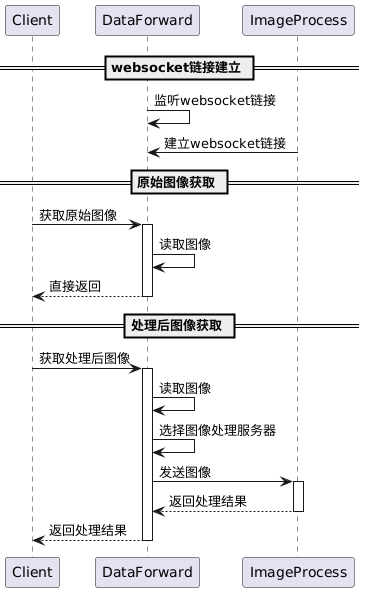
\includegraphics[width=0.7\textwidth]{websocket.png}  % 图片文件路径,设置宽度为页面宽度的80%
    \caption{系统架构图}  % 图片标题
    \label{fig:websocket}
\end{figure}

如上图所示,系统的操作可分为以下几个阶段:

\begin{enumerate}
    \item WebSocket 链接建立:\\ 在系统初始化阶段,DataForward 服务器持续监听潜在的 WebSocket 连接请求。各个 ImageProcess 服务器主动向 DataForward 服务器发起 WebSocket 连接。这些持久化连接是后续数据传输和命令控制的基础,标志着图像处理服务节点的注册与在线状态。
    \item 原始图像获取:\\ 当 Client 发起获取原始图像的请求时,该请求被路由至 DataForward。DataForward 在接收到请求后,将执行图像读取操作,并直接将原始图像数据返回给 Client。在此过程中,DataForward 主要充当一个数据代理角色,不涉及复杂的图像处理逻辑。
    \item 处理后图像获取:\\ 对于 Client 请求获取处理后图像的场景,DataForward 作为核心协调者发挥作用。
    \begin{itemize}
        \item DataForward 首先会读取待处理的原始图像。
        \item DataForward 实现了基于主备机制的智能路由策略:它会优先选择当前被标记为"主"的 ImageProcess 服务器进行任务转发。
        \item 若当前的主 ImageProcess 服务器检测到离线状态,DataForward 将立即触发自动故障转移(Automatic Failover)机制,将下一个可用的备用 ImageProcess 服务器提升为新的主服务器,以确保服务的连续性。
        \item 随后,DataForward 将图像数据发送给选定的 ImageProcess 服务器进行处理。
        \item ImageProcess 完成处理后,会将结果返回给 DataForward。DataForward 将处理后的图像结果转发回 Client。
    \end{itemize}
\end{enumerate}

\section{代码实现}

\subsection{main.rs}

该文件中包含了整个 DataForward 服务器的主要逻辑。它负责初始化日志模块、 Actix Web 应用程序,设置路由,并启动 WebSocket 服务器以处理来自 ImageProcess 服务器的连接。

\subsection{web\_socket\_actor.rs}

该文件定义了 WebSocketActor 结构体,它实现了 Actix Web 的 Actor 特性。WebSocketActor 负责处理与 ImageProcess 服务器的 WebSocket 连接,包括接收消息、发送消息以及管理连接状态。

\subsection{api.rs}

该文件定义了 API 路由和处理函数。它包括处理原始图像获取和处理后图像获取的 HTTP 路由。每个路由都对应一个处理函数,这些函数负责根据要求获取图像数据并返回给客户端。